% A LaTeX template for EXECUTIVE SUMMARY of the MSc Thesis submissions to 
% Politecnico di Milano (PoliMi) - School of Industrial and Information Engineering
%
% S. Bonetti, A. Gruttadauria, G. Mescolini, A. Zingaro
% e-mail: template-tesi-ingind@polimi.it
%
% Last Revision: October 2021
%
% Copyright 2021 Politecnico di Milano, Italy. NC-BY

\documentclass[11pt,a4paper,twocolumn]{article}

%------------------------------------------------------------------------------
%	REQUIRED PACKAGES AND  CONFIGURATIONS
%------------------------------------------------------------------------------
% PACKAGES FOR TITLES
\usepackage{titlesec}
\usepackage{color}

% PACKAGES FOR LANGUAGE AND FONT
\usepackage[utf8]{inputenc}
\usepackage[english]{babel}
\usepackage[T1]{fontenc} % Font encoding

% PACKAGES FOR IMAGES
\usepackage{graphicx}
\graphicspath{{Images/}} % Path for images' folder
\usepackage{eso-pic} % For the background picture on the title page
\usepackage{subfig} % Numbered and caption subfigures using \subfloat
\usepackage{caption} % Coloured captions
\usepackage{transparent}

% STANDARD MATH PACKAGES
\usepackage{amsmath}
\usepackage{amsthm}
\usepackage{bm}
\usepackage[overload]{empheq}  % For braced-style systems of equations

% PACKAGES FOR TABLES
\usepackage{tabularx}
\usepackage{longtable} % tables that can span several pages
\usepackage{colortbl}

% PACKAGES FOR ALGORITHMS (PSEUDO-CODE)
\usepackage{algorithm}
\usepackage{algorithmic}

% PACKAGES FOR REFERENCES & BIBLIOGRAPHY
\usepackage[colorlinks=true,linkcolor=black,anchorcolor=black,citecolor=black,filecolor=black,menucolor=black,runcolor=black,urlcolor=black]{hyperref} % Adds clickable links at references
\usepackage{cleveref}
\usepackage[square, numbers, sort&compress]{natbib} % Square brackets, citing references with numbers, citations sorted by appearance in the text and compressed
\bibliographystyle{plain} % You may use a different style adapted to your field

% PACKAGES FOR THE APPENDIX
\usepackage{appendix}

% PACKAGES FOR ITEMIZE & ENUMERATES 
\usepackage{enumitem}

% OTHER PACKAGES
\usepackage{amsthm,thmtools,xcolor} % Coloured "Theorem"
\usepackage{comment} % Comment part of code
\usepackage{fancyhdr} % Fancy headers and footers
\usepackage{lipsum} % Insert dummy text
\usepackage{tcolorbox} % Create coloured boxes (e.g. the one for the key-words)
\usepackage{stfloats} % Correct position of the tables

%-------------------------------------------------------------------------
%	NEW COMMANDS DEFINED
%-------------------------------------------------------------------------
% EXAMPLES OF NEW COMMANDS -> here you see how to define new commands
\newcommand{\bea}{\begin{eqnarray}} % Shortcut for equation arrays
\newcommand{\eea}{\end{eqnarray}}
\newcommand{\e}[1]{\times 10^{#1}}  % Powers of 10 notation
\newcommand{\mathbbm}[1]{\text{\usefont{U}{bbm}{m}{n}#1}} % From mathbbm.sty
\newcommand{\pdev}[2]{\frac{\partial#1}{\partial#2}}
% NB: you can also override some existing commands with the keyword \renewcommand

%----------------------------------------------------------------------------
%	ADD YOUR PACKAGES (be careful of package interaction)
%----------------------------------------------------------------------------


%----------------------------------------------------------------------------
%	ADD YOUR DEFINITIONS AND COMMANDS (be careful of existing commands)
%----------------------------------------------------------------------------


% Do not change Configuration_files/config.tex file unless you really know what you are doing. 
% This file ends the configuration procedures (e.g. customizing commands, definition of new commands)
% Set the geometric layout of the document
\usepackage{geometry}
\geometry{
  top=3cm,
  left = 2.0cm,
  right = 2.0cm,
  bottom=2cm,
  headheight= 2cm,
  headsep= 0cm,
}
\raggedbottom 

% Create color bluePoli (-> manuale grafica coordinata:  https://www.polimi.it/fileadmin/user_upload/il_Politecnico/grafica-coordinata/2015_05_11_46xy_manuale_grafica_coordinata.pdf)
\definecolor{bluePoli}{cmyk}{0.4,0.1,0,0.4}

% Custom theorem environments
\declaretheoremstyle[
  headfont=\color{bluePoli}\normalfont\bfseries,
  bodyfont=\color{black}\normalfont\itshape,
]{colored}

\captionsetup[figure]{labelfont={color=bluePoli}} % Set colour of the captions
\captionsetup[table]{labelfont={color=bluePoli}} % Set colour of the captions
\captionsetup[algorithm]{labelfont={color=bluePoli}} % Set colour of the captions

\theoremstyle{colored}
\newtheorem{theorem}{Theorem}[section]
\newtheorem{proposition}{Proposition}[section]

% Enhances the features of the standard "table" and "tabular" environments.
\newcommand\T{\rule{0pt}{2.6ex}}
\newcommand\B{\rule[-1.2ex]{0pt}{0pt}}

% Algorithm description
\newcounter{algsubstate}
\renewcommand{\thealgsubstate}{\alph{algsubstate}}
\newenvironment{algsubstates}{
    \setcounter{algsubstate}{0}%
    \renewcommand{\STATE}{%
    \stepcounter{algsubstate}%
    \Statex {\small\thealgsubstate:}\space}
    }{}
    
% Custom theorem environment
\newcolumntype{L}[1]{>{\raggedright\let\newline\\\arraybackslash\hspace{0pt}}m{#1}}
\newcolumntype{C}[1]{>{\centering\let\newline\\\arraybackslash\hspace{0pt}}m{#1}}
\newcolumntype{R}[1]{>{\raggedleft\let\newline\\\arraybackslash\hspace{0pt}}m{#1}}

% Custom itemize environment
\setlist[itemize,1]{label=$\bullet$}
\setlist[itemize,2]{label=$\circ$}
\setlist[itemize,3]{label=$-$}
\setlist{nosep}

% Set separation of columns 
\setlength{\columnsep}{30pt}

% Create command for background pic
\newcommand\BackgroundPic{% Adding background picture
	\put(230,358){
		\parbox[b][\paperheight]{\paperwidth}{%
			\vfill
			\centering
			\transparent{0.4}
			
\includegraphics[width=0.5\paperwidth]{raggiera_polimi.eps}%
			\vfill
}}}

% Set indentation
\setlength\parindent{0pt}

% Custom title commands
\titleformat{\section}
{\color{bluePoli}\normalfont\Large\bfseries}
{\color{bluePoli}\thesection.}{1em}{}
\titlespacing*{\section}
{0pt}{2ex}{1ex}

\titleformat{\subsection}
{\color{bluePoli}\normalfont\large\bfseries}
{\color{bluePoli}\thesubsection.}{1em}{}
\titlespacing*{\subsection}
{0pt}{2ex}{1ex}

% Custom headers and footers
\pagestyle{fancy}
\fancyhf{}
      
\fancyfoot{}
\fancyfoot[C]{\thepage} % page
\renewcommand{\headrulewidth}{0mm} % headrule width
\renewcommand{\footrulewidth}{0mm} % footrule width

\makeatletter
\patchcmd{\headrule}{\hrule}{\color{black}\hrule}{}{} % headrule
\patchcmd{\footrule}{\hrule}{\color{black}\hrule}{}{} % footrule
\makeatother

% -> Create the header
\chead[C]{
\centering
\begin{tcolorbox}[arc=0pt, boxrule=0pt, colback=bluePoli!60, width=\textwidth, colupper=white]
    \textbf{Executive summary} \hfill \textbf{\author}  
\end{tcolorbox}
}

% Insert here the info that will be displayed into your Title page 
% -> title of your work
\renewcommand{\title}{4WIS4WID mobile robot autonomous navigation in agricultural setting using End-to-End Reinforcement Learning}
% -> author name and surname
\renewcommand{\author}{Paolo Ginefra}
% -> advisor name and surname
\newcommand{\advisor}{prof. M. Restelli, prof. S. Mentasti, prof. M. Matteucci}
% IF AND ONLY IF you need to modify the co-supervisors you also have to modify the file Configuration_files/title_page.tex (ONLY where it is marked)
\newcommand{\firstcoadvisor}{Name Surname} % insert if any otherwise comment
%\newcommand{\secondcoadvisor}{Name Surname} % insert if any otherwise comment
% -> academic year
\newcommand{\YEAR}{2024-2025}

%-------------------------------------------------------------------------
%	BEGIN OF YOUR DOCUMENT
%-------------------------------------------------------------------------
\begin{document}

%-----------------------------------------------------------------------------
% TITLE PAGE
%-----------------------------------------------------------------------------
% Do not change Configuration_files/TitlePage.tex (Modify it IF AND ONLY IF you need to add or delete the Co-advisors)
% This file creates the Title Page of the document
% DO NOT REMOVE SPACES BETWEEN LINES!

\twocolumn[{\begin{@twocolumnfalse}

\AddToShipoutPicture*{\BackgroundPic}

\hspace{-0.6cm}
\includegraphics[width=0.6\textwidth]{logo_polimi_ing_indinf.eps}

\vspace{-1mm}
\fontsize{0.3cm}{0.5cm}\selectfont \bfseries \textsc{\color{bluePoli} Report for the project}\\

\vspace{-0.2cm}
\Large{\textbf{\color{bluePoli}{\title}}}\\

\vspace{-0.2cm}
\fontsize{0.3cm}{0.5cm}\selectfont \bfseries \textsc{\color{bluePoli} Laurea Magistrale in \course}\\

\vspace{-0.2cm}
\fontsize{0.3cm}{0.5cm} \selectfont \bfseries Author: \textsc{\textbf{\author}}\\

\vspace{-0.4cm}
\fontsize{0.3cm}{0.5cm}\selectfont \bfseries Advisor: \textsc{\textbf{\advisor}}\\

% if only ONE co-advisor is present:
\vspace{-0.4cm}
\fontsize{0.3cm}{0.5cm}\selectfont \bfseries Co-advisor: \textsc{\textbf{\firstcoadvisor}}\\
% if more than one co-advisors are present:
%\vspace{-0.4cm}
%\fontsize{0.3cm}{0.5cm}\selectfont \bfseries Co-advisors: \textsc{\textbf{\firstcoadvisor}}\textsc{\textbf{\secondcoadvisor}}\\

\vspace{-0.4cm}
\fontsize{0.3cm}{0.5cm}\selectfont \bfseries Academic year: \textsc{\textbf{\YEAR}}

\small \normalfont

\vspace{11pt}

\centerline{\rule{1.0\textwidth}{0.4pt}}

\vspace{15pt}
\end{@twocolumnfalse}}]

\thispagestyle{plain} % In order to not show the header in the first page


%%%%%%%%%%%%%%%%%%%%%%%%%%%%%%
%%     THESIS MAIN TEXT     %%
%%%%%%%%%%%%%%%%%%%%%%%%%%%%%%

%-----------------------------------------------------------------------------
% INTRODUCTION
%-----------------------------------------------------------------------------
\section{Introduction}
\label{sec:introduction}
This project explores a fundamental question in agricultural robotics: can Task 1 of the Field Robot Event 2025 be solved using an end-to-end Reinforcement Learning (RL) approach with the Rockerbot platform? Rather than following the traditional Sense-Plan-Act paradigm employed by most competing teams, this work investigates whether a deep RL policy can learn to navigate autonomously through crop rows by processing raw sensor data and directly outputting control commands.

The motivation for this approach is twofold. First, end-to-end learning has demonstrated remarkable success in various robotic control tasks, potentially offering a more adaptive and generalizable solution compared to hand-crafted algorithms. Second, this project serves as the author's first substantial real-world application of the RL framework, making the learning process itself a primary objective alongside task completion.

The challenge is particularly compelling due to Rockerbot's unique 4 Wheels Independent Steering 4 Wheels Independent Drive (4WIS4WID) kinematic configuration. This system provides exceptional maneuverability but introduces significant control complexity through motion constraints and kinematic discontinuities. Traditional control approaches must carefully manage these constraints, while an RL agent must discover effective control strategies through exploration.

The project follows a structured three-phase plan: developing a high-fidelity simulation environment, training an RL policy in simulation, and bridging the sim-to-real gap for physical deployment. However, substantial technical challenges emerged early in development. Building the simulation environment in Isaac Lab consumed approximately two-thirds of the total time budget, primarily due to the need for custom LIDAR implementation and the framework's developmental limitations. Consequently, the project advanced through only the first phase and partially into the second, stopping at level 4 of the proposed developer curriculum.

Despite not reaching physical deployment, this work yields valuable contributions. The developed simulation framework provides a reusable platform for future agricultural robotics research, and the extensive experimentation process has generated concrete insights into practical RL application. The project demonstrates both the potential and the challenges of applying end-to-end RL to structured agricultural tasks, offering a foundation for continued development toward competition-ready autonomous navigation.


\section{The Task}
\label{sec:task}

\subsection{Field Robot Event 2025}
The Field Robot Event (FRE) is an international competition where university teams design, build, and test autonomous agricultural robots. The event challenges the robots to perform realistic farming tasks such as navigating crop rows, recognising plants and obstacles, detecting weeds, and mapping fields. It aims to promote innovation in agricultural robotics by providing students with practical experience in robotics, AI, and engineering applied to sustainable farming. The competition includes several tasks testing precision, navigation, object recognition, and a freestyle challenge showcasing novel capabilities.
To make the competition more challenging, each robot \textbf{cannot use any form of satellite-based positioning (GPS, ...)}.
The 2025 edition was held in Milan, Italy, running from June 9 to 12.

\subsection{FRE25 Task 1 - Autonomous Navigation}
\label{subsec:task1}
Among the 5 tasks of the competition, the first has been selected as the most suitable to be solved with Reinforcement Learning. That is because it is both the least structured one (other tasks involve object recognition and some form of counting) and the one more closely related to control (something in which RL typically excels).

The Task takes place in a cultivated field, among rows of small corn plants, each with a height of approximately 40/45 cm. Each row is approximately 20 m long, and it is about 75 cm apart from the others. The rows are slightly curved, but they all have roughly the same shape. The plants are evenly spaced along the rows, but sometimes they can be missing.

The robot starts in one of the corners of the field, and it needs to navigate the rows alternating between going forward and backwards. At the beginning of the task, a sequence of instructions is provided to the robot. Each instruction $i \in S_{com} = \{1,2\} \times \{L, R\}$ is a tuple that express what to do at the end of a row. It specifies how many rows to skip and the direction of the turn. The direction assumes that the robot faces the end of the row. The sequence of instructions $I \in \bigcup_{i=1}^{\infty}S_{com}^i$ has no specified length. The layout of the task can be found displayed in Figure \ref{fig:task1}.

\begin{figure}
    \centering
    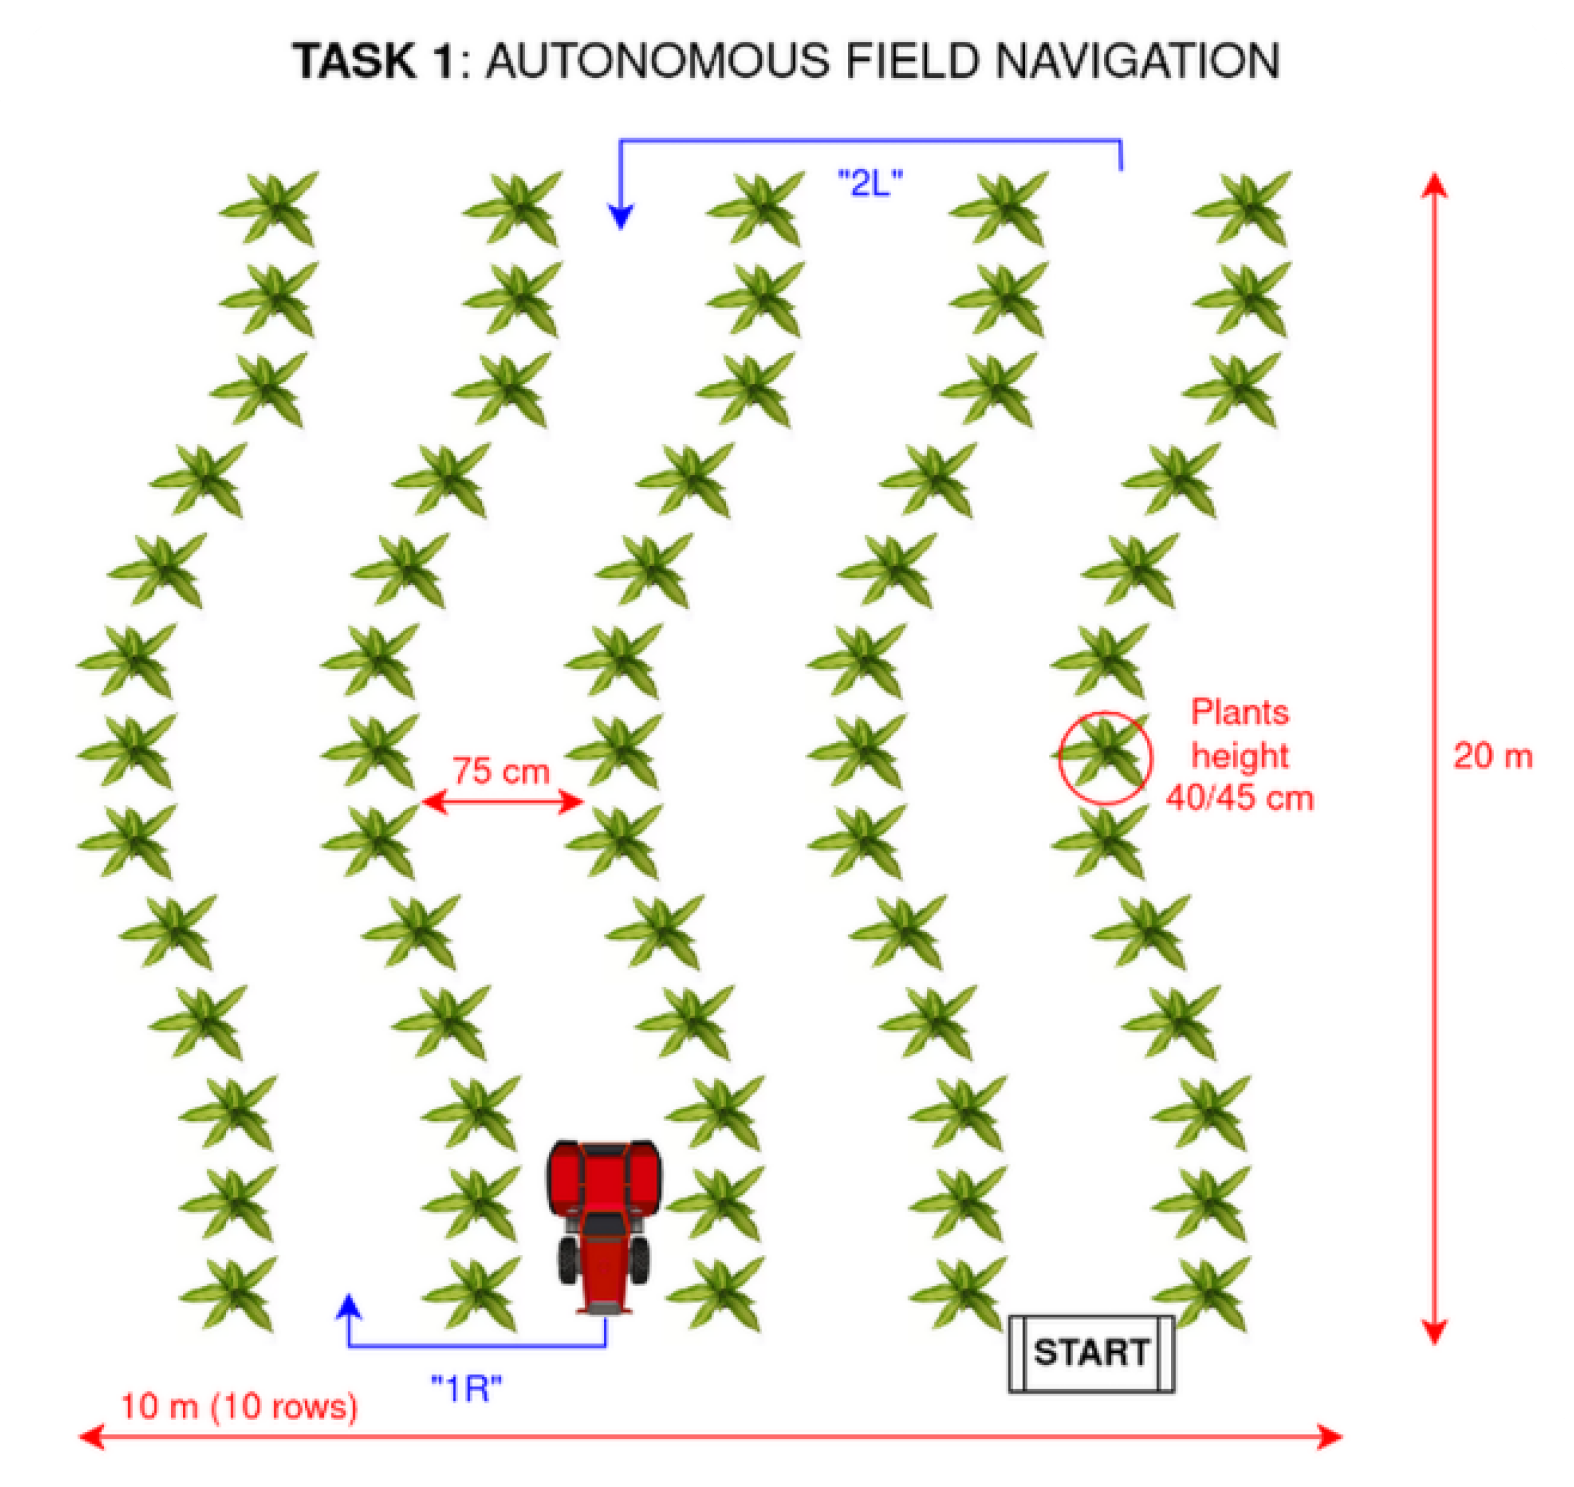
\includegraphics[width=\linewidth]{Multidisciplinary_Project_Report//Images/Task1Schema.png}
    \caption{A diagram displaying the configuration of Task 1}
    \label{fig:task1}
\end{figure}

\subsection{Rockerbot}
\label{sec:rockerbot}

The robot developed by Politecnico di Milano for the Field Robot Event is called Rockerbot. It was upgraded to its current form for the 2024 edition, and it remained mostly unchanged for the 2025 one. A picture of Rockerbot in the crop field of Task 1 of the FRE24 can be found in Figure \ref{fig:rockerbot}.

Rockerbot is a mobile robot with 4 driving wheels. What makes this robot unique is the fact that each wheel can rotate on its zenithal axis, and each yaw can be controlled independently. This gives rise to the \textbf{4 Wheels Independent Steering 4 Wheels Independent Drive (4WIS4WID) kinematic \cite{4WIS4WID}}.

Rockerbot is equipped with two encoders per wheel: a position encoder for the yaw and a velocity encoder for the angular velocity along the spinning axis. Furthermore, it features two planar LIDARs, one located at the front and one at the rear, with the plane of perception parallel to the ground. The encoders and the LIDARs are the only means of perception available.

\begin{figure}
    \centering
    \includegraphics[width=1\linewidth]{Multidisciplinary_Project_Report/Images/Rockerbot.png}
    \caption{A photo of Rockerbot in the field of Task 1 of the FRE 24}
    \label{fig:rockerbot}
\end{figure}

\section{The 4WIS4WID kinematic}

\begin{figure}
    \centering
    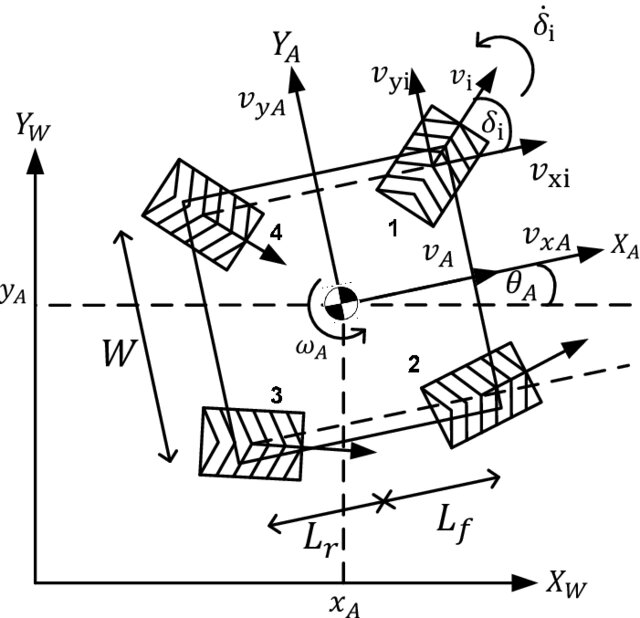
\includegraphics[width=1\linewidth]{Multidisciplinary_Project_Report/Images/4WISskematic.png}
    \caption{The schematic of the 4WIS4WID kinematic taken from \cite{4WISschematic}}
    \label{fig:4WIS}
\end{figure}

This peculiar kinematic is really flexible, and it theoretically allows the robot to achieve all 3 of its planar degrees of freedom. All the following notation is depicted in Figure \ref{fig:4WIS} and it is in line with \cite{4WIS4WID} and \cite{4WISschematic}.

The robot coordinate frame $\{X_A, Y_A\}$ is attached to the robot's center of mass (CoM), which moves with a linear velocity $\mathbf{v}_A = [v_{xA}, v_{yA}]^T$ and an angular velocity $\omega_A$. 
Each wheel $i \in \{1, 2, 3, 4\}$ has a steering angle $\delta_i$ and linear velocity $\vec{v}_i = [v_{xi}, v_{yi}]^T$ expressed in the vehicle frame. 
The front and rear axles are separated by a wheelbase of $L_f + L_r$, while the track width is $W$. 
The world coordinate frame $\{X_W, Y_W\}$ is fixed to the ground, and $\theta_A$ denotes the vehicle's heading angle with respect to the global $X_W$ axis. 
The front wheels (1, 2) and rear wheels (3, 4) can each steer independently, allowing omnidirectional motion.

Unfortunately, Rockerbot imposes some constraints:
\begin{itemize}
    \item Due to cable management, each wheel can only rotate 180°: 
    $$
    -\pi/2 \leq \delta_i \leq \pi/2 \quad \forall i \in \{1, \cdots, 4\}
    $$
    \item Due to physical limitations of the motors, each wheel can reach a limited velocity and a limited zenithal angular velocity:
    $$
    |\vec{v}_i| \leq v_{max} \quad \forall i \in \{1, \cdots, 4\}
    $$
    $$
    \dot{\delta}_i \leq \dot{\delta}_{max} \quad \forall i \in \{1, \cdots, 4\}
    $$
\end{itemize}

These constraints, especially the first one, heavily restrict the feasible trajectories in the $C = \{[v_{xA}, v_{yA}, \omega_A]^T|v_{xA}, v_{yA}, \omega_A \in \mathbb{R}\}$ control space because they introduce many discontinuities.

Controlling the robot in the $C$ space will be referred to as \textbf{Full Rigid Body Kinematic (FRBK)}. That's because it harnesses all the degrees of freedom left after a rigid body assumption.

A 4WIS4WID robot control can be further constrained to obtain many more kinematics:
\begin{itemize}
    \item \textbf{Double Ackermann (2DoF)} - the robot must always be oriented as its velocity vector:
    $$
    v_{yA} = 0
    $$

    \item \textbf{Crab (2DoF)} - the robot can only translate:
    $$
    \omega_{A} = 0
    $$

    \item \textbf{Pivot (1DoF)} - the robot can only rotate in place:
    $$
    v_{xA} = v_{yA} = 0
    $$
\end{itemize}

A partial order $\leq$ between kinematics can be constructed as follows:

Let $A$ and $B$ be two kinematics, than $A \leq B$ i.f.f. all the robot's poses $[x_a, y_a, \theta_a, \delta_1, v_1, \cdots, \delta_4,v_4]^T$ reachable using $A$ can be reached using $B$. A diagram showing how the kinematics are ordered can be found in Figure \ref{fig:poset}.

\begin{figure*}
    \centering
    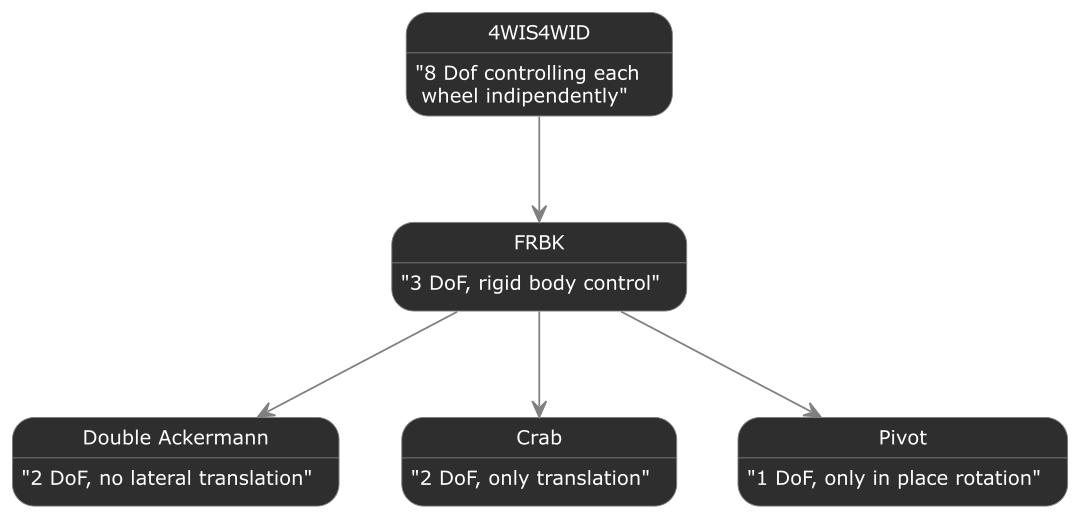
\includegraphics[width=1\linewidth]{Multidisciplinary_Project_Report/Images/poset.png}
    \caption{A diagram showing the "$\leq$" ordering of kinematics. If two kinematics $A$ and $B$ are connected by an arrow pointing at $B$, then $B \leq A$"}
    \label{fig:poset}
\end{figure*}

\section{Traditional Solution}
\label{sec:trad}
FRE's Task 1 is typically addressed using a more traditional approach, following the Sense Plan Act paradigm. of Probabilistic Robotics. More in detail, one can follow 2 strategies:
\begin{itemize}
    \item \textbf{SLAM based}: Using Simultaneous Localisation and Mapping algorithms \cite{DurrantWhyte2006SimultaneousLA} \cite{ProbabilisticRobotics}, one can use the standard navigation pipeline similar to the one implemented in the ROS package Nav2 \cite{nav2}.
    \item \textbf{SLAMless}: due to hardware limitations, SLAM might not be feasible. In that case, new, simpler custom solutions must be implemented. This was the route taken by the Politecnico's team for both FRE24 and FRE25. The solution splits the problem into three parts. \textbf{In row Navigation} is performed by extracting the relative row direction from the LIDAR scans using Computer Vision techniques, which is then followed by a PID controller. \textbf{End of Row Detection} is based on counting heuristics, while the \textbf{Turning} is performed in open-loop, counting the skipped rows using heuristics. 
\end{itemize}

\section{Project Plan}
The ultimate goal of this project is to determine how close to a competition-ready solution can be achieved using End-to-End Reinforcement Learning. This means that the agent has to be responsible for the totality of the strategy, taking only the sensor's readings as input and directly outputting the controls. If one's goal was to achieve the best competition performance in the least amount of engineering time, an end-to-end approach wouldn't be advisable. Adding inductive bias by integrating already developed solutions (like the row direction extractor of the previous approaches) would massively speed up training and allow for finer developer control.
Another alternative could have been to develop a solution by collecting human demonstrations directly in the field and train a policy using imitation learning \cite{ImitationLearning}. 

The ambitious goal of this project could not be tackled all at once; thus, it has been partitioned into the following subgoals:
\begin{enumerate}
    \item Building a simulation of FRE25 task 1
    \item Develop an RL policy in simulation
    \item Address the Sim2Real gap and deploy the policy on Rockerbot
\end{enumerate}

The very nature of this project could not allow for a linear progression between stages, since the experience and requirements of a future phase inevitably call for modification in a previous one. Unfortunately, due to time constraints, \textbf{this project could not reach the third phase}, and it stopped in the middle of the second one.

\section{Simulation}
\subsection{Simulator choice}
For the simulation, Nvidia's Isaac Lab \cite{IsaacLab} has been chosen.
Isaac Lab is an open-source framework for robotics research that leverages GPU acceleration through its foundation on NVIDIA Isaac Sim. The framework addresses common challenges in robotics research by providing a unified platform for diverse methodologies, including reinforcement learning, imitation learning, and motion planning. Its simulation capabilities utilise PhysX for physics computation and ray-tracing technologies for sensor modelling, aiming to reduce the gap between simulated and real-world robot behaviour. The framework's architecture emphasises modularity and extensibility, including pre-configured robot models and experimental environments that can be adapted to various research needs. Isaac Lab supports integration with multiple learning frameworks and can be deployed across different computational infrastructures, from local workstations to distributed cloud systems.
Isaac Lab is a powerful tool, but it is still in its developmental stage. This meant that it cannot yet accommodate a large variety of needs. Even though the final performance of the simulation is outstanding, reaching peaks of around \textbf{3000 simulation steps per second}, the development of the simulation consumed around 2/3 of the total time budget.

\subsection{Simulation Landscape}
The simulation has been developed starting from the actual CAD model of Rockerbot. Each wheel is equipped with its own couple of controllers that follow a mass-spring-damper model. The target yaw and rotational effort can be set for each wheel independently.

The ground is currently modelled by a rigid plane, and each plant is represented by a 3D model.

The strength of Isaac Lab lies in its ability to simulate many environments in parallel. In the simulation, there are $N_e$ environment. Each environment has one robot and $p = r \cdot \rho$ plants, where $r$ is the number of rows and $\rho$ is the number of plants per row.

\subsection{Row generation}
The shape of the rows is determined by a stochastic process
\[
S(t, \Theta_s): [0,1] \to \mathbb{R}^2,
\]
whose realizations define continuous curves in the plane.

In the \( i \)-th environment, at the beginning of each episode, 
the parameters \( \theta_{si} \) are sampled. 
The corresponding curve \( S(t, \theta_{si}) \) describes 
all the rows of the \( i \)-th environment for that episode.

The position of the \( j \)-th plant in the \( k \)-th row,
expressed in the environment reference frame, is given by:
\begin{align*}
    t_{ijk} &= \tfrac{j-1}{\rho-1}, \\
    \varepsilon &\sim \mathcal{N}(\vec{0}, I\sigma_p), \nonumber\\
    Plant_{ijk} &= S(t_{ijk}, \theta_{si}) + [0, k \Delta_r] + \varepsilon, \nonumber
\end{align*}
with \( i \in \{1,\!\dots,\!N_e\} \), 
\( j \in \{1,\!\dots,\!\rho\} \),
\( k \in \{1,\!\dots,\!r\} \),
and \( \Delta_r \in \mathbb{R}^+ \) the distance between rows.

In the simulator, \( S \) is implemented by interpolating a set of 
points with a cubic spline~\cite{Spline}. 
The control points are the parameters of the process. 
Let \( l_r \) be the row length and \( c_r \in \mathbb{N} \) 
the number of control points:
\begin{align*}
    \Theta &= \big((0, Y_1),\, 
        (l_r \tfrac{1}{c_r-1}, Y_2),\, \dots,\,
        (l_r, Y_{c_r})\big), \nonumber\\
    \vec{Y} &\sim \mathcal{N}(\vec{0}, I\sigma_c), \nonumber\\
\end{align*}
then 
$$
S(t, \Theta) = \text{spline}(t, \Theta)
$$

This implementation choice has been made for simplicity's sake, but future versions might implement Gaussian Processes for finer control on the rows' shape.

\subsection{Command Buffer}
The task requires the robot to follow certain commands as explained in Section \ref{subsec:task1}. In the i-th environment, at the beginning of each episode, the instruction sequence $I_i$ of fixed length $l_c \in \mathbb{N}$ is generated randomly and uniformly, and it is stored in a queue $Q(q):\{0,1\} \to S_{com}$. The queue always returns the current command and moves to the next every rising front of its control signal $q$. When the queue has reached its last command, it ignores the control.

\subsection{Waypoints}
The simulation has a waypoint system that traces the path the robot should follow. In the i-th environment, after the path parameters, $\theta_{si}$ are sampled and the command sequence $I_i$ is generated, the waypoints are set up to have $\rho_w$ evenly spaced waypoints in the middle of the relevant rows and one waypoint per row skipped during turns. The in-row waypoints start and end slightly outside the rows on the x direction by a padding of $p_{in}$. The turning waypoints have the same y coordinate as the last plant on the relevant side of the row and an x that is $p_{t}$ away in the relevant direction. The waypoints are arranged in a snake-like pattern.
The waypoints are ordered, and they can only be reached in the right sequence. For a waypoint to be reached, the robot must be at a distance of less than $\varepsilon_w$ and it must be the first unreached waypoint of the order. The only reachable waypoint at a time will be referenced as the next waypoint.

\subsection{LIDARs}
Isaac Lab has integrated simulated LIDARs based on the ray tracing capabilities of Nvidia's GPUs. Unfortunately, in the current version 
of Isaac Lab, this feature is available only for sensing static objects. Since the plants need to change position at each environment reset, they are intrinsically dynamic. This was one of the major setbacks of the project because it required a \textbf{from-scratch implementation of planar LIDARs}. Early attempts at ray tracing showed unsatisfactory performance, which led to the usage of ray marching techniques \cite{Raymarching}. This algorithm allows to find the point of intersection of a ray and a shape very efficiently.  In 2D Raymarching, shapes are described by a Signed Distance Field $sdf(\vec{x}):\mathbb{R}^2\to\mathbb{R}$ that describes the signed distance of a generic point $\vec{x} \in \mathbb{R}^2$, where a negative distance means that $\vec{x}$ is inside the shape. These functions are then used in the collision finding algorithm, as given a scene described by $\{sdf_i|i\in{1, \cdots, k}\}$ and any point $\vec{\hat{x}}$ which is outside all the shapes, surely all the points in $A_{\vec{\hat{x}}} = \{\vec{x}\in\mathbb{R}^2: ||\vec{\hat{x}}-\vec{x}||_2 \leq \min_{i}sdf_i(\vec{\hat{x}}) \}$ will be outside all the shapes. Given a ray described by a direction $\vec{d}\in\mathbb{R}^2, ||\vec{d}||_2 = 1$, and a starting point $\vec{x}^{(0)} \in \mathbb{R}^2$, the algorithm keep iterating $\vec{x}^{(n)} = \vec{x}^{(n-1)} + \vec{d} \min_{i}sdf_i(\vec{x}^{(n-1)})$ until either the maximum number of iterations $n_{lidar}$ is reached,  $\min_{i}sdf_i(\vec{x}^{(n)})<\varepsilon_{lidar}$ or $||x^{(n)} - x^{(0)}||_2 > d_{lmax}$. This procedure can be used to simulate a LIDAR by simply repeating the procedure for each ray, and since each ray is independent, this can easily be parallelised. $n_{rays}$ rays are simulated for each LIDAR. For the plants, a simple circular signed distance function has been implemented, where given a plant position $\vec{p} \in \mathbb{R}^2$ and a plant radius $r_{plant} \in \mathbb{R}^+$, $sdf_p(\vec{x})=||\vec{x} - \vec{p} ||_2 - r_{plant}$. This model is quite simplistic, but with the required smoothing and anomaly detection can be quite faithful to the actual Rockerbot's LIDARs. Another approximation is that in the simulation, the robot has only one 360° unobstructed LIDAR instead of the two of the actual robot, but once again, with the due pre-processing, the simulated configuration can be a faithful approximation.

\subsection{Termination Conditions}
For each environment, the episode terminates when at least one of the following conditions is met:
\begin{itemize}
    \item \textbf{Plant collision}: the robot collides with a plant
    \item \textbf{Out of bound}: the distance between the robot and the next waypoint is greater than the waypoint reached tolerance $\varepsilon_w$ plus the distance between the next and the last (meaning the one before the next) waypoint.
    \item \textbf{Time out}: the episode has exhusted the time budget $t_{sim}$
    \item \textbf{Completion}: The robot has reached all the waypoints
\end{itemize}

\section{Reinforcement Learning Problem Formulation}
FRE25 task 1 can be framed as a continuous state, observations, and actions \textbf{Partially Observable Markov Decision Process (POMDP) \cite{POMDPS}}. What follows is a possible general formulation of the problem as a POMDP. In the next section, all the tweaks necessary to achieve a working solution are discussed in greater detail. 

\subsection{States}
The States of the POMDP are made up of:
\begin{itemize}
    \item All the plants' positions in the current episode
    \item The robot's position, orientation, and the yaw and speed of each wheel
\end{itemize}

All of these are, at best, accessible to the robot through noisy measurements.

\subsection{Observations}
The robot can observe the states via the wheels' position and velocity encoders and the LIDAR. The robot is also aware of the current command in the Command Buffer.

\subsection{Actions}
The actions performable by the agent vary depending on the chosen kinematics, but in general, they are the robot's controls. For the goal 4WIS4WID kinematic, the actions would be the angle and the velocity targets for each wheel. The control signal of the Command Buffer is also controlled by the policy.

\subsection{Reward}
A reward function should reflect the goal of the learning process. In the simulation, the simplest way to access a policy's performance is through the number of reached waypoints. 

\section{RL Proposed Solution}
To solve the problem, the chosen algorithm is Proximal Policy Optimisation \cite{Schulman2017ProximalPO} due to its widespread adoption in similar applications, relatively straightforward implementation compared to trust region methods, native support for both continuous and discrete action spaces without architectural modifications, and demonstrated robustness to hyperparameter variations across diverse problem domains. It is also natively integrated in Isaac Lab through many RL libraries, the chosen one is Stable Baselines 3 \cite{raffin2021stable}

\subsection{Proposed Developer Curriculum}
To assert how close to a full end-to-end solution one can get with this setup, the following procedure has been followed during the development process:
\begin{itemize}
    \item If, by tuning hyperparameters, the performance does not seem to improve, simplify the problem
    \item When a satisfactory level of performance is reached, increase the difficulty of the problem
\end{itemize}

By experimenting with this procedure, the following difficulty sequence has been identified, ordered by task difficulty in decreasing order:
\begin{enumerate}
    \item \textbf{The Full Task} - 4WIS4WID, Command buffer control, Skip up to 2 rows,
    \item \textbf{The Task with a Rigid Body} - FRBK, Command buffer control, Skip up to 2 rows
    \item \textbf{The Task translating} - Crab, Command buffer control, Skip up to 2 rows
    \item \textbf{The Task translating without skipping} - Crab, Command buffer control, Skip up to 1 row
    \item \textbf{Just plain navigation} - Crab, Automatic Command buffer control, Skip up to 1 row
\end{enumerate}
The Crab kinematic has been chosen as the baseline as it has proven to be a fruitful strategy by other competitors in the FRE24. The time budget allowed the current implementation to reach only level 4, but all the tools are in place to move further. \textbf{The rest of this section refers to the current implementation}.

\subsection{Crab Differential Actions}
The constraints of the crab kinematic implies $\delta = \delta_i, i\in\{1, \cdots, 4\}$. Thus, the control variables are just $\delta \in [-\pi/2, \pi/2]$ and a throttle $f \in [-1,1]$. Taking inspiration from classic control theory, a differential control has been chosen. The policy will then act by choosing $\dot{\delta}$ and $\dot{f}$. This has two main advantages, both confirmed by empirical evidence:
\begin{itemize}
    \item It makes the learning process easier and more stable, gaining the same advantages as feedback control,
    \item It makes it easier to enforce physical constraints like $\dot{\delta}_{max}$ 
\end{itemize}

\subsection{Encoders}
With a Crab kinematic a single current yaw $\delta = \frac{1}{4}\sum_{i=1}^{4}\delta_i$ is fed to the policy as the current steering. 

\subsection{Accumulator-Based Memory Model}
Since the Markov assumption is violated, the policy needs to retain information about its previous states and actions. The standard solution is to implement a policy model with memory (RNN, LSTM, GRU, $\cdots$). These architectures are notoriously slow to train due to their intrinsic sequential nature and thus not very parallelizable. This is in stark contrast to the massively parallel implementation of Isaac Lab, and it soon became apparent that these kinds of policies are not feasible in the current setup.

Furthermore, despite the partial observability, the task doesn't seem to show any crucial long-horizon time dependence. This led to the implementation of an accumulator-based memory model that tries to get closer to a Markovian scenario by constructing the continuous hidden state $\vec{h}\in\mathbb{R}^{d_h}$. The policy will receive $\vec{h}$ as an additional observation, and it will act on it by choosing $\dot{\vec{h}}$. This is inspired by the odometry usually performed in mobile robot navigation. $\vec{h}$ essentially functions as a scratchpad for the policy, and as such, it can be used for interpretability purposes.

Moreover, to allow for higher-order control and since the command buffer functions on the rising front of its control signal, the previous actions performed by the policy are also fed as observations.

\subsection{Command Buffer Parity}
To facilitate the alternating movement, the parity of the current command's index in its sequence is also fed to the policy as an observation.

\subsection{Action Discretization}
The choice of differential controls also allows for strong discretisation of the action space, further simplifying the problem. In particular, the robot kinematic controls can be reduced to categorical values as follows: $\dot{\delta}, \dot{f} \in \{-1, 0, 1\}$. The Command Buffer control $q$ can just be binary and the hidden state differential can also become categorical as $\dot{\vec{h}}\in \{-1, 1\}^{n_h}$ 

\subsection{Reward shaping}
Only rewarding the model with a +1 whenever it reaches a waypoint resulted as too sparse for efficient learning to happen. The current reward function is a linear combination of many factors:
\begin{itemize}
    \item Whether a waypoint is reached in the current simulation step,
    \item The projected velocity of the robot $\vec{v}$ in the global reference frame onto the line connecting the robot to the next waypoint 
    \item A penalty for plant collisions
    \item A penalty for time-out
    \item A penalty for being out of bounds
    \item A penalty for stepping the command buffer
    \item A penalty proportional to the absolute difference of the current row number and the index of the current command in the command buffer
    \item a penalty proportional to the distance to the next waypoint
    
\end{itemize}

The actual coefficients of the combination can be found in the code repository.

\section{Results}

\subsection{Final Configuration}
After 339 training runs totalling 487.29 hours of training experimentation, the following configuration represents the current best-performing setup for Task 1 navigation at curriculum level 4. This solution can consistently follow up to 7 commands, effectively navigating up to 8 crop rows, more than enough for the FRE25 Task 1.

\subsubsection{Environment Parameters}
The simulation environment parameters are listed in Table \ref{tab:sim_params}.

\begin{table}[h]
\centering
\caption{Simulation Environment Parameters}
\label{tab:sim_params}
\small
\begin{tabular}{|l|r|l|}
\hline
\textbf{Parameter} & \textbf{Value} & \textbf{Unit} \\
\hline
\multicolumn{3}{|c|}{\textit{Timing}} \\
\hline
Decimation & 4 & - \\
Simulation dt & 1/120 & s \\
Episode length ($t_{sim}$) & 300.0 & s \\
\hline
\multicolumn{3}{|c|}{\textit{Command Buffer}} \\
\hline
Commands length & 8 & - \\
Max rows & 1 & - \\
\hline
\multicolumn{3}{|c|}{\textit{Path Generation}} \\
\hline
Row spacing ($\Delta_r$) & 1.2 & m \\
Control points ($c_r$) & 10 & - \\
Path length ($l_r$) & 3.0 & m \\
Control point noise std ($\sigma_c$) & 0.15 & m \\
Plant noise std ($\sigma_p$) & 0.03 & m \\
\hline
\multicolumn{3}{|c|}{\textit{Waypoints}} \\
\hline
Waypoints per row ($\rho_w$) & 3 & - \\
Reached tolerance ($\varepsilon_w$) & 0.35 & m \\
End of row  ($p_{in}$) & 0.4 & m \\
Extra waypoint padding ($p_t$) & 0.8 & m \\
\hline
\multicolumn{3}{|c|}{\textit{Plants}} \\
\hline
Plants per path ($\rho$) & 10 & - \\
Plant radius ($r_{plant}$) & 0.22 & m \\
\hline
\multicolumn{3}{|c|}{\textit{LiDAR Sensor}} \\
\hline
Rays per robot ($n_{rays}$) & 40 & - \\
Max distance ($d_{lmax}$) & 1.0 & m \\
Tolerance ($\varepsilon_{lidar}$) & 0.01 & m \\
Max raymarching steps ($n_{lidar}$) & 100 & - \\
\hline
\end{tabular}
\end{table}

\subsubsection{Reward Function Parameters}
The reward function weights are shown in Table \ref{tab:reward_params}.

\begin{table}[h]
\centering
\caption{Reward Function Parameters}
\label{tab:reward_params}
\small
\begin{tabular}{|l|r|}
\hline
\textbf{Component} & \textbf{Weight} \\
\hline
Waypoint reward base & 100.0 \\
Velocity toward waypoint scale & 0.5 \\
Timeout penalty & -100.0 \\
Plant collision penalty & -100.0 \\
Out of bounds penalty & -100.0 \\
Command step penalty & 0.0 \\
Command index penalty scale & -1.0 \\
Distance penalty scale & 1.0 \\
Total reward scale & 0.1 \\
\hline
\end{tabular}
\end{table}

\subsubsection{Policy and Training Configuration}
The PPO algorithm hyperparameters and network architecture are detailed in Table \ref{tab:training_params}.

\begin{table}[h]
\centering
\caption{PPO Training Parameters}
\label{tab:training_params}
\small
\begin{tabular}{|l|r|}
\hline
\textbf{Parameter} & \textbf{Value} \\
\hline
\multicolumn{2}{|c|}{\textit{PPO Hyperparameters}} \\
\hline
Learning rate & 2e-4 \\
Gamma (discount factor) & 0.99 \\
GAE lambda & 0.95 \\
Clip range & 0.2 \\
Entropy coefficient & 0.01 \\
Value function coefficient & 2.0 \\
Max gradient norm & 1.0 \\
\hline
\multicolumn{2}{|c|}{\textit{Training Setup}} \\
\hline
Number of environments ($N_e$) & 128 \\
Steps per environment & 256 \\
Batch size & 256 \\
Number of epochs & 10 \\
\hline
\multicolumn{2}{|c|}{\textit{Network Architecture}} \\
\hline
Policy network & [256, 128, 64] \\
Value network & [256, 128, 64] \\
Activation function & ReLU \\
\hline
\multicolumn{2}{|c|}{\textit{Action Space}} \\
\hline
Steering action & \{-1, 0, +1\} \\
Throttle action & \{-1, 0, +1\} \\
Step command action & \{0, 1\} \\
Number of Hidden states ($d_h$) & 4 \\
\hline
\multicolumn{2}{|c|}{\textit{Observation Space}} \\
\hline
Current steering angle & 1 \\
LiDAR readings & 40 \\
Command buffer state & 3 \\
Past control actions & 3 \\
Hidden accumulators & 4 \\
\textbf{Total observation dim} & \textbf{51} \\
\hline
\end{tabular}
\end{table}

\subsection{Training Performance}
The current configuration achieves the following performance metrics:
\begin{itemize}
    \item \textbf{Training time from scratch}: Approximately 1 hour
    \item \textbf{Time to first row completion}: Approximately 2 minutes of training
    \item \textbf{Total training runs}: 339 runs across all experiments
    \item \textbf{Total computational time}: 487.29 hours (20.30 days)
    \item \textbf{Simulation speed}: Up to 3000 steps per second
\end{itemize}

The training process demonstrated that observation and action space design had greater impact on learning success than hyperparameter tuning. The differential action space combined with the accumulator-based memory model proved essential for achieving stable learning in this partially observable navigation task.

\subsection{Qualitative Lessons}
In the current state of the project, the most valuable product of this project is not yet the control policy, but the long list of mistakes and lessons learned on how to effectively interact with the Reinforcement Learning framework. What follows is a list of qualitative heuristics learned during development in no particular order:
\begin{itemize}
    \item \textbf{Hyperparameters are not all you need}: tuning hyperparameters can be helpful but with PPO it becomes secondary. Once in one of the many broad areas of stability of the algorithm, changing the observations, actions and reward has a much greater effect
    \item \textbf{Avoid Partially Observable Software Development}: Once a headless training run is going, the behaviour of the simulation can only be observed through logs. The better the logging tools, the easier it is to gain insight into what is actually happening and the easier it is to spot problems sooner
    \item \textbf{Model Architecture is not that important}: Compared to other fields of machine learning, the actual size of the network does not impact performance that much.
    \item \textbf{Pre-training helps}: Once a model architecture and the observations/actions domains are identified, training from scratch can be wasteful, while starting from a previous checkpoint and overriding key hyperparameters/reward structure can be a major speed-up.
    \item \textbf{Remember to also test at scale}: When dealing with a highly vectorised environment, some issues may arise only when multiple environments are run together.
    \item \textbf{Make sure that the POMDP formulation describes a doable task}: Features like teleoperation and observation plotting can make the difference in understanding the weak points of the current formulation.
    \item \textbf{Always make structured hypotesis when tuning hyperparameters}: Searching in a huge space can be daunting and confusing, thus some structure in the experimentation is needed 

    
\end{itemize}

\section{Future Work}

While this project establishes a foundation for RL-based agricultural navigation, several critical research directions remain unexplored. What follows is a list of ideas and proposals on what the next step for this project could be.

\subsection{Empirical Validation Through Ablation Studies}

The current implementation introduces several design choices: accumulator-based memory, action discretisation, and multi-component reward shaping. Due to time constraints, those have been greedily optimised towards better performance without a more thorough empirical analysis. A sequence of ablation studies could lead to more structured knowledge about each element's contribution. 

\paragraph{Memory Architecture Comparison}
A controlled comparison between memory mechanisms is needed:
\begin{itemize}
    \item \textbf{Baseline}: No memory (current observations only)
    \item \textbf{Frame stacking}: Concatenate last $k$ observations
    \item \textbf{Accumulator}: Current implementation with $\dot{\vec{h}}$ control
    \item \textbf{LSTM/GRU}: Recurrent architectures despite computational cost
\end{itemize}
Each variant should be trained with identical hyperparameters for $n \geq 5$ random seeds, measuring convergence speed, sample efficiency, final success rate, and computational overhead.

\paragraph{Action Space Design}
The discretization to $\{\dot{\delta}, \dot{f}\} \in \{-1, 0, 1\}$ dramatically constrains the control space. An ablation study should compare:
\begin{itemize}
    \item Continuous differential actions: $\dot{\delta}, \dot{f} \in [-1, 1]$
    \item Coarse discretization: $\{-1, 0, 1\}$ (current)
    \item Fine discretization: $\{-1, -0.5, 0, 0.5, 1\}$
    \item Direct control: $\delta, f$ without differential formulation
\end{itemize}
Metrics should include final performance, learning stability (variance across seeds), and interpretability of learned policies.

\paragraph{Reward Decomposition Analysis}
The reward function (Section 8.6) linearly combines seven terms with manually tuned coefficients. A principled approach requires:
\begin{enumerate}
    \item \textbf{Component ablation}: Remove each reward term individually to identify critical components
    \item \textbf{Coefficient sensitivity}: Vary each coefficient by orders of magnitude ($0.1\times, 1\times, 10\times$)
    \item \textbf{Automated tuning}: Apply reward scaling methods or population-based training
    \item \textbf{Sparse baseline}: Compare against waypoint-only rewards to quantify the benefit of shaping
\end{enumerate}

\subsection{Baseline Comparisons and Benchmarking}

The current work lacks a performance baseline. Some possible candidates could be the traditional approaches listed in \ref{sec:trad}.

\paragraph{Alternative Learning Methods}
\begin{itemize}
    \item \textbf{Behavioral cloning}: Train supervised policy from expert demonstrations (classical controller trajectories)
    \item \textbf{Other RL algorithms}: SAC, TD3 for continuous control comparison
\end{itemize}

Each method should be evaluated on identical test scenarios with metrics including: success rate, average waypoints reached, trajectory smoothness, computational requirements, and sample efficiency (for learning methods).

\subsection{Generalization and Robustness Analysis}

Current training and evaluation use the same distribution of environments. Rigorous evaluation requires:

\paragraph{Systematic Generalization Tests}
\begin{itemize}
    \item \textbf{Row curvature}: Train on $\sigma_c = 0.5$, test on $\sigma_c \in \{0.1, 1.0, 2.0\}$
    \item \textbf{Plant density}: Train on $\rho = 20$, test on $\rho \in \{10, 15, 25, 30\}$
    \item \textbf{Row spacing}: Train on $\Delta_r = 0.75$m, test on $\Delta_r \in \{0.6, 0.9\}$m
    \item \textbf{Missing plants}: Train with 0\% missing, test with \{10\%, 20\%, 30\%\} randomly missing
    \item \textbf{Sensor noise}: Add graduated noise to LIDAR and encoder readings
\end{itemize}

\paragraph{Domain Randomization}
Implement training with randomized parameters (the standard sim-to-real approach) and measure whether generalization improves at the cost of peak performance on training distribution.

\subsection{Scaling the Difficulty Curriculum}

The project stopped at level 4 of 5 in the proposed curriculum. Completing the progression requires:

\paragraph{Level 3: Multi-row Skipping}
Enable skipping up to 2 rows during turns. This requires:
\begin{itemize}
    \item More complex waypoint counting in the accumulator state
    \item Extended command buffer reasoning
    \item Potentially longer episodes for exploration
\end{itemize}

\paragraph{Level 2: Full Rigid Body Kinematic}
Remove the $\omega_A = 0$ constraint, allowing simultaneous translation and rotation. Challenges include:
\begin{itemize}
    \item Expanded action space: $[v_{xA}, v_{yA}, \omega_A]$
    \item More complex kinematic constraints
    \item Risk of kinematic singularities during learning
\end{itemize}

\paragraph{Level 1: Full 4WIS4WID Control}
The ultimate goal: independent control of all four wheels. This requires addressing:
\begin{itemize}
    \item 8-dimensional action space (4 angles, 4 velocities)
    \item Discontinuities from $\delta_i \in [-\pi/2, \pi/2]$ constraints
    \item Kinematic coordination between wheels
    \item Potentially hierarchical control policies
\end{itemize}

\subsection{Sim-to-Real Transfer Strategy}

Physical deployment requires explicit bridging of the reality gap:

\paragraph{Systematic Noise Modeling}
\begin{itemize}
    \item Characterize real sensor noise (LIDAR, encoders) through data collection
    \item Model actuation delays and inaccuracies
    \item Implement these as randomization parameters in simulation
\end{itemize}

\paragraph{Sim-to-Real Techniques}
Explore methods such as:
\begin{itemize}
    \item Domain randomization with gradually increasing variance
    \item Fine-tuning with small amounts of real-world data
    \item Residual RL: RL policy correcting classical controller
\end{itemize}

\subsection{Interpretability and Failure Analysis}

Understanding policy behavior is essential for debugging and trust:

\paragraph{Visualization Tools}
\begin{itemize}
    \item Attention maps: Which LIDAR rays most influence decisions?
    \item Accumulator state trajectories: What information is stored in $\vec{h}$?
    \item Action distribution evolution: How does the policy's action selection change spatially?
\end{itemize}

\paragraph{Systematic Failure Characterization}
Collect and categorize failure modes:
\begin{itemize}
    \item Where in the episode do failures occur? (start, mid-row, turns)
    \item What environment features correlate with failure? (curvature, plant gaps)
    \item Are failures deterministic or stochastic for the same scenario?
\end{itemize}


\section{Conclusion}

This project investigated whether end-to-end Reinforcement Learning could solve the autonomous navigation challenge of FRE25 Task 1 using Rockerbot. Physical deployment was not achieved within the available timeframe, as approximately two-thirds of the time budget was consumed by simulation development.

The main technical outcome is a functional Isaac Lab simulation environment that models the task scenario, including procedural crop row generation, custom ray marching-based LIDAR implementation for dynamic objects, and Rockerbot's 4WIS4WID kinematic constraints. The simulation runs at approximately 3000 steps per second.

An RL policy was developed that can navigate crop rows using the Crab kinematic. After 339 training runs totaling 487.29 hours, the current configuration trains from scratch in about one hour and completes the first row after approximately two minutes of training. Key design choices included differential action spaces, accumulator-based memory to address partial observability, and structured reward shaping.

The development process revealed practical considerations for applying RL to robotics problems. Observation and action space design had greater impact than hyperparameter tuning, comprehensive logging proved essential for understanding training behavior, and pre-training from checkpoints accelerated development. The time required for simulation infrastructure should not be underestimated when working with emerging frameworks.

The simulation framework and trained policies provide a foundation for advancing through the remaining curriculum levels toward full 4WIS4WID control and eventually addressing the sim-to-real gap. While the original goal was not reached, the project demonstrates that RL approaches are applicable to agricultural navigation tasks and documents the practical challenges encountered in this process.


%---------------------------------------------------------------------------
%  BIBLIOGRAPHY
%---------------------------------------------------------------------------
% Remember to insert here only the essential bibliography of your work
\bibliography{bibliography.bib} % automatically inserted and ordered with this command 

\end{document}